

% trial .tex file %
\documentclass[9pt]{article}  % specifies document class (article) and point size (10pt)
\usepackage{graphicx}
\usepackage{polski}
\usepackage[utf8]{inputenc}
\usepackage{sidecap}
\usepackage{wrapfig}
\usepackage{subfig}
\usepackage{amsmath}
\usepackage{float}
\usepackage{enumerate}
\usepackage{listings}
\usepackage{listings}
\usepackage{color}

\definecolor{dkgreen}{rgb}{0,0.6,0}
\definecolor{gray}{rgb}{0.5,0.5,0.5}
\definecolor{mauve}{rgb}{0.58,0,0.82}

\lstset{frame=tb,
  language=R,
  aboveskip=3mm,
  belowskip=3mm,
  showstringspaces=false,
  columns=flexible,
  basicstyle={\small\ttfamily},
  numbers=none,
  numberstyle=\tiny\color{gray},
  keywordstyle=\color{blue},
  commentstyle=\color{dkgreen},
  stringstyle=\color{mauve},
  breaklines=true,
  breakatwhitespace=true,
  tabsize=3
}


\begin{document}               % starts document
\author{Michał Kubica}
\title{Modele Liniowe \\ Raport nr 1}       
\maketitle                     % constructs big, fancy title

\section{Zadanie 1}            % makes a section header

    Wygenerowano 100 wektorów losowych z rozkładu dwuwymiarowego normalnego $N \left( 0, I \right)$ poniższym kodem w R:

    \begin{lstlisting}
  X = matrix(0,100,2)
  for (i in 1:100){
    X[i,] = rnorm(2)
  }
    \end{lstlisting}    
    
    A następnie zaznaczono je na płaszczyźnie.
    
    \begin{figure}[H]
      \centering
      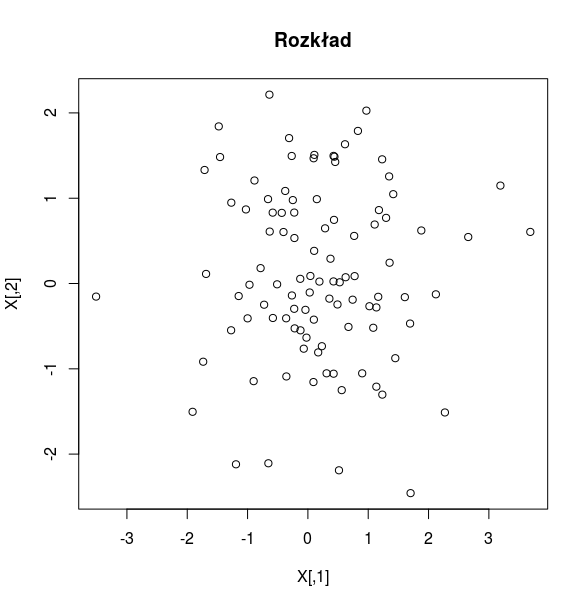
\includegraphics[width=0.6\textwidth]{zad1.png}
      \caption {}
    \end{figure}
    

    
    \section{Zadanie 2}
    
    W tym zadaniu należało przekształcić liniowo otrzymane wektory losowe tak, aby miały one rozkład o średniej $\mu = {4 \choose 2}$ i macierzy kowiariancji $\Sigma$. Korzystając z własności i wzorów na liście zadań zadanie sprowadziło się do wyznaczenia takiej macierzy A, aby spełnione było równanie macierzone: 
    $ \Sigma = AA^T$.
    Macierz A wyznaczono na dwa sposoby: metodą Choleskiego(funkcji \textit{chol}) oraz rachunkiem algebraicznym jak w poniższym przykładzie.\newline
    \newline
        
    $ \Sigma = 
      \left( \begin{array}{cc}
      1 & 0.9  \\
      0.9 & 1  \\
      \end{array} \right)
    =   
      \left( \begin{array}{cc}
      a & b  \\
      c & d  \\
      \end{array} \right)      
      \left( \begin{array}{cc}
      a & c  \\
      b & d  \\
      \end{array} \right)   
    =
      \left( \begin{array}{cc}
      a^2 + b^2 & ac + bd  \\
      ac + bd & c^2 + d^2  \\
      \end{array} \right)  
    $
    \newline
    
    $$
    \left\{ \begin{array}{l}
    a^2+b^2 = 1 \\
    ac+bd = 0,9 \\
    c^2+d^2 = 1 \\
    \end{array} \right.
    $$
    \newline
    
    przyjmując b = 0 otrzymujemy \newline
    
      A = \left( \begin{array}{cc}
      1 & 0  \\
      0,9 & \sqrt{0.19}  \\
      \end{array} \right)  
      \newline
      \newline
    
    Dla każdej z trzech róznych macierzy kowariancji zaznaczono na płaszczyźnie przekształconą chmurę wektorów oraz wygenerowane wektory za pomocą funcji \textit{rmvnorm}.

    
    \subsection{$ \Sigma = 
          \left( \begin{array}{cc}
      1 & 0.9  \\
      0.9 & 1  \\
      \end{array} \right)}
      
    \begin{figure}[H]
      \centering
      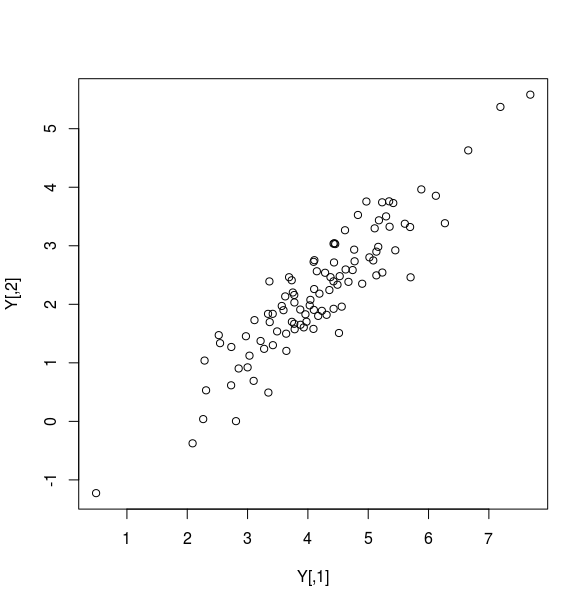
\includegraphics[width=0.5\textwidth]{21.png}
      \caption {Przekształcona chmura wektorów}
    \end{figure}
    
        \begin{figure}[H]
      \centering
      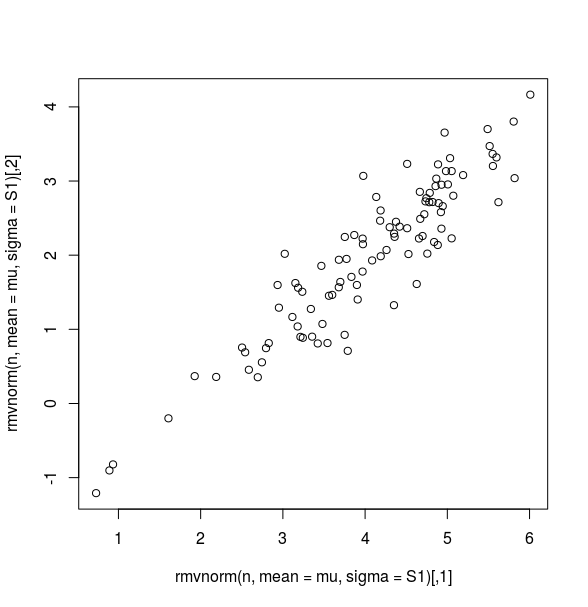
\includegraphics[width=0.5\textwidth]{21m.png}
      \caption {Wylosowane 100 wektorów losowych za pomocą rvrnorm}
    \end{figure} 
      
      
    Na obu wykresach widać wyraźną zależność liniową między wektorami losowymi. Wyniki się zgadzają z przewidywaniami związanymi z postacią macierzy kowariancji.
      
      
      
    \subsection{$ \Sigma = 
          \left( \begin{array}{cc}
      1 & -0.9  \\
      -0.9 & 1  \\
      \end{array} \right)}
      
      
    \begin{figure}[H]
      \centering
      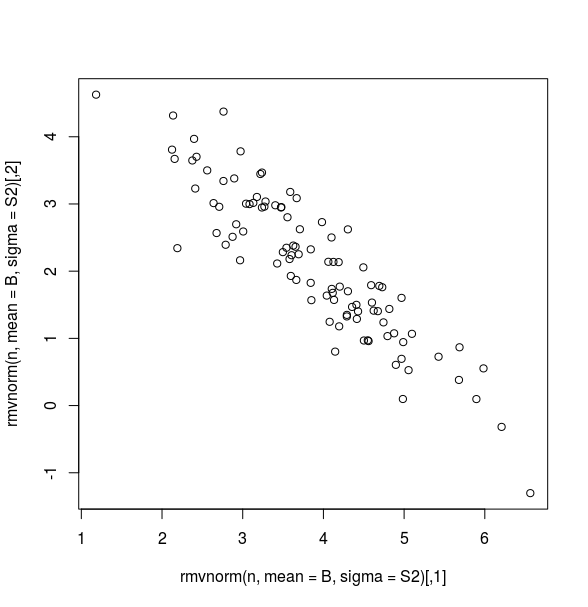
\includegraphics[width=0.5\textwidth]{22.png}
      \caption {Przekształcona chmura wektorów}
    \end{figure}
      
          \begin{figure}[H]
      \centering
      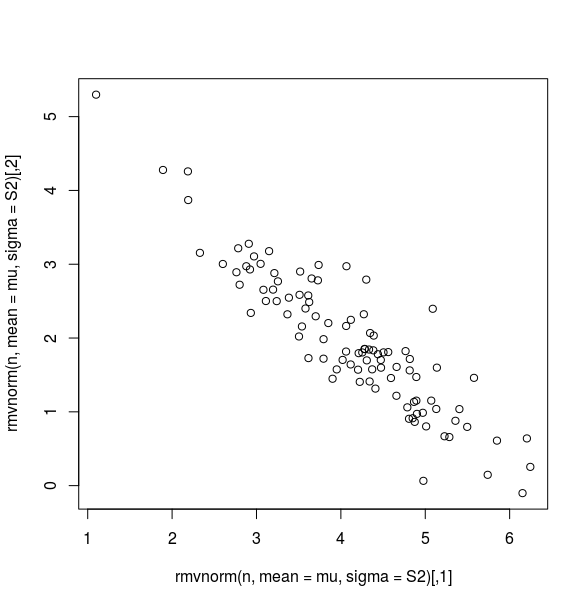
\includegraphics[width=0.5\textwidth]{22m.png}
      \caption {Wylosowane 100 wektorów losowych za pomocą rvrnorm}
    \end{figure} 
    
        Na obu wykresach widać wyraźną odwrotną zależność liniową między wektorami losowymi. Wyniki się zgadzają z przewidywaniami związanymi z postacią macierzy kowariancji.
      
    \subsection{$ \Sigma = 
          \left( \begin{array}{cc}
      9 & 0  \\
      0 & 1  \\
      \end{array} \right)}
      
      
    \begin{figure}[H]
      \centering
      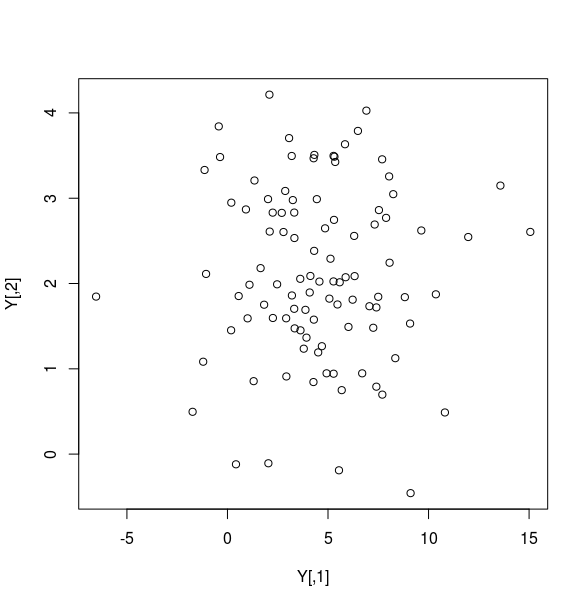
\includegraphics[width=0.5\textwidth]{23.png}
      \caption {Przekształcona chmura wektorów}
    \end{figure}
    
        \begin{figure}[H]
      \centering
      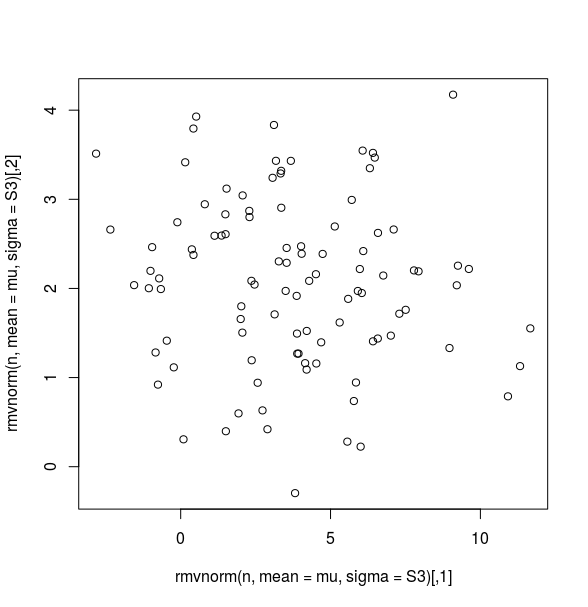
\includegraphics[width=0.5\textwidth]{23m.png}
      \caption {Wylosowane 100 wektorów losowych za pomocą rvrnorm}
    \end{figure} 
    
    W tym przypadku nie ma jakiejkolwiek zależności liniowej między wektorami, ale to jednak nie wyklucza istnienia zależności nieliniowej.\newline \newline
    
    
    \subsection{Kod R}
    
    \begin{lstlisting}
S1 = matrix(c(1, 0.9, 0.9, 1), 2, 2)
S2 = matrix(c(1, -0.9, -0.9, 1), 2, 2)
S3 = matrix(c(9, 0, 0 ,1), 2, 2)

sqrt(0.19)
A1 = t(chol(S1))
A2 = t(chol(S2))
A3 = t(chol(S3))

mu = c(4,2)

Y = t(A1%*%t(X)+mu)
plot(Y)
plot(rmvnorm(n, mean=mu, sigma=S1 ))

Y = t(A2%*%t(X)+mu)
plot(Y)
plot(rmvnorm(n, mean=mu, sigma=S2 ))

Y = t(A3%*%t(X)+mu)
plot(Y)
plot(rmvnorm(n, mean=mu, sigma=S3 ))
    \end{lstlisting}   

    

    

  \section{Zadanie 3}
  
  
  Za pomocą funkcji \textit{rnorm} wygenerowano 200 wektorów losowych z rozkładu wielowymiarowego normalnego $N \left(0,I_{100x100} \right)$. Korzystając z własności przekształcenia liniowego i metody Choleskiego wyznaczono macierz $A$ taką, że $\tilde{X} = AX$ oraz $\tilde{X} \sim N\left(0,\Sigma \right) $, gdzie $$
  
  
  $$
    \mathbf{\Sigma} =
    \left( \begin{array}{cccc}
    1 & 0.9 & \ldots & 0.9\\
    0.9 & 1 & \ldots & 0.9 \\
    \vdots & \vdots & \ddots & 0.9 \\
    0.9 & 0.9 & 0.9 & 1 
    \end{array} \right)
  $$
  
  Ze względu na trudności, związane z wizualizacją wektorów losowych o wymiarze 100, zweryfikowano poprawność wygenerowanych wektorów losowych wyliczając średnią, rysując histogram próbkowych wariancji współrzędnych wektora $\tilde{X}$ oraz próbkowych kowariancji między różnymi współrzędnymi tego wektora.
  
  Wyliczona średnia wynosi: -0.003316602
  
  
          \begin{figure}[H]
      \centering
      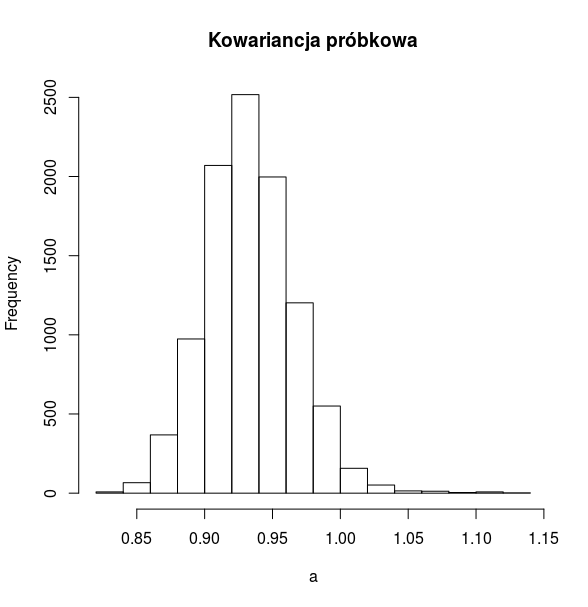
\includegraphics[width=0.8\textwidth]{32.png}
      \caption {Histogram próbkowych kowariancji}
    \end{figure} 
    
    
    Kowariancja próbkowa waha się od 0.9 do 1, a więc jest to zgodne z oczekiwaniami i postacia macierzy kowariancji. A więc na podstawie wyliczenia średniej i powyższego wykresu można powiedzieć, że wketory został← wygenerowane poprawnie.
    
    
    
    
        \subsection{Kod R}
    
    \begin{lstlisting}

my_rmvnorm=function(mu,Sigma){
  r = length(mu)
  L = t(chol(Sigma)) 
  Z = rnorm(r)
  return(L %*% Z + mu)
}

n = 200
m = 100

Sigma = diag(m)
mu = rep(0,m)

X = matrix(0,m,n)
for(i in 1:n){
 X[,i] = my_rmvnorm(mu, Sigma)
}
X
X = t(X)

x = rep(0,m)
for(i in 1:m){
  x[i] = mean(X[,i])
}
x
mean(x)
mean(X)

sigma = matrix(0.9,m,m) + 0.1*diag(m)

A = t(chol(sigma))
Y = A%*%t(X)

Y
plot(t(Y))

hist(var(Y), main='Histogram próbkowych wariancji')


a = matrix(0, 100, 100)
for (i in 1:100){
  for (j in 1:100){
    a[i,j] = cov(Y[i,], Y[j,])
  }
}
a
hist(a, main='Kowariancja próbkowa')
    \end{lstlisting}   
  



\end{document}  







